\section{Evaluation}
\label{sec:eval}

We evaluate on a testbed whose sensing age is measured rather than assumed. A home
node and \ifblind a\else an Atlas\fi{} workstation-class node with GV100 GPUs run
the controller, which probes real GPU occupancy and admits real CUDA workers while
a competing tenant drives capacity. The fabric carrying this control plane is
characterized in the companion paper~\cite{companion}. Unless noted we report the
mean and a $t$-based $95\%$ confidence interval over independent repeats. Four
questions organize the study. \textbf{(Q1)} What is the sensing age $D$ that
governs Prop.~\ref{prop:bound}. \textbf{(Q2)} Does Algorithm~\ref{alg:adaptive}
stay polite while beating a fixed budget when it holds a self-imposed budget.
\textbf{(Q3)} Does that hold under real time-varying contention, and where does it
fail. \textbf{(Q4)} Does the value $\tfrac12 r(D)$ of Thm.~\ref{thm:limit} hold at
the controller level, and does it also bind a learned controller.

\subsection{Sensing age and the violation bound (Q1)}
\label{sec:eval-detection}
The sensing age has two measured parts. A read-only \texttt{nvidia-smi} probe
costs $27$ to $33$\,ms at the median. The end-to-end delay from launching a real
GPU load until it is visible as utilization above the $40\%$ floor is
$\mathbf{2.46}$\,s over 10 thermally guarded repeats on a GV100, with median
$2.48$ and range $2.29$ to $2.61$. CUDA start-up dominates that figure, not the
poll. Which value applies depends on the question. Detecting whether a newly
admitted pod is productive pays the full start-up cost, while probing pods that
are already running costs only the poll. One epoch is a single completion-gated
admission decision whose measured mean duration is about $1.1$\,s, so the
$2.46$\,s start-up age is $D\approx2$ to $3$ epochs, which we sweep in Q4, and
the $27$\,ms poll is below one epoch for running pods. Substituting into
Prop.~\ref{prop:bound} makes $D$ a first-order term in achievable politeness. A
guest that admits aggressively with large $\alpha$ pays for it in over-admission
scaled by this measured start-up delay.

\subsection{Politeness under a self-imposed budget (Q2)}
\label{sec:eval-e2e}
We burst $B$ jobs under three policies against a self-imposed politeness budget
$C$, measuring goodput in tasks per second and the over-budget fraction $\rho$,
the share of epochs with concurrency above $C$. The policies are \emph{naive},
which submits up to the hard cap, \emph{static}, a fixed submit rate, and
\emph{aimd}, the trackable branch of Algorithm~\ref{alg:adaptive}. To isolate the
policy from the exogenous scheduling and image-pull variance of the shared
cluster, which produced three pre-registered nulls in situ and is reported as
such, we run on a controlled node with local-process workers and no scheduler or
registry jitter. The design was pre-registered with randomized interleaved trial
order and four repeats per cell, at two scales.

Table~\ref{tab:e8} reports it. Algorithm~\ref{alg:adaptive} holds the budget
exactly at both scales, with $\rho=0$, while delivering $1.72$ times (GPU) and
$3.18$ times (CPU) the goodput of a fixed rate at the same politeness. At the GPU
scale it also matches naive's goodput without exceeding the budget. At the CPU
scale, where naive over-admits flagrantly at $\rho=0.95$, naive buys about twice
the goodput and Algorithm~\ref{alg:adaptive} trades that headroom for politeness.
Both pre-registered hypotheses hold with disjoint intervals at both scales. This
isolates the admission rule on a controlled node, and the full pod-scheduling path
is verified separately in \S\ref{sec:impl}. Here the budget is self-imposed, so
\S\ref{sec:eval-contended} removes that assumption.

\begin{table}[t]
\centering
\caption{Goodput against politeness under a self-imposed budget, 4 repeats, mean
with $95\%$ interval. Algorithm~\ref{alg:adaptive} holds the budget at a fixed
rate's politeness with $1.7$ to $3.2$ times its goodput.}
\label{tab:e8}
\small
\begin{tabular}{llcc}
\toprule
scale & policy & goodput (tasks/s) & over-budget $\rho$ \\
\midrule
\multirow{3}{*}{GPU, $C{=}2$}
 & naive  & $0.0538\pm0.0003$ & $0.54\pm0.01$ \\
 & aimd   & $0.0539\pm0.0001$ & $0.00\pm0.00$ \\
 & static & $0.0313\pm0.0000$ & $0.00\pm0.00$ \\
\midrule
\multirow{3}{*}{CPU, $C{=}8$}
 & naive  & $0.5779\pm0.0062$ & $0.95\pm0.00$ \\
 & aimd   & $0.2928\pm0.0029$ & $0.00\pm0.00$ \\
 & static & $0.0920\pm0.0002$ & $0.00\pm0.00$ \\
\bottomrule
\end{tabular}
\end{table}

\subsection{Politeness under real contention (Q3)}
\label{sec:eval-contended}
The harder question is politeness when capacity is genuinely scarce. We manufacture
controlled contention on a two-GPU node with $C{=}2$. A competing tenant occupies
$c(t)\in\{0,1\}$ GPUs on a fixed profile, so the guest's available capacity
$a(t)=C-c(t)$ is exogenous, time-varying and measured by the prober through a
per-GPU process census subject to the sensing age of Q1. Two profiles bracket the
space. \emph{Square} load is a period-$2\tau$ wave modelling slowly varying or
scheduled neighbours, and \emph{poisson} load is memoryless on and off arrivals,
the adversarial case. Alongside goodput and $\rho$ we measure harm to the
neighbour as the competitor's completed work relative to its undisturbed baseline.
The study was pre-registered with randomized interleaved order and four seeds per
cell.

Table~\ref{tab:e9} reports a sharper picture than the self-imposed budget did.
Under structured load Algorithm~\ref{alg:adaptive} is the polite and efficient
knee. It reaches $1.41$ times a fixed rate's goodput, $0.091$ against
$0.064$\,tasks/s with disjoint intervals, at $\rho=0.15$, which is a quarter of
naive's $0.64$, and it spares the neighbour, retaining $76\%$ of its throughput
against naive's $62\%$. The target $\epsilon$ and switch level $\theta$ were fixed
before the runs. Host policy penalizes persistently under-utilized requests rather
than momentary dips, so $\epsilon$ between $0.1$ and $0.2$ is the tolerable share
of under-utilized epochs, and the measured $0.15$ sits inside it. Naive's higher
goodput of $0.101$ is bought entirely at the neighbour's expense, since it
over-admits two-thirds of the time and takes $38\%$ of the competitor's
throughput.

Under memoryless load feedback breaks even and we report it. Goodput of $0.062$ is
statistically indistinguishable from the fixed rate's $0.064$ with overlapping
intervals, and over-admission is worse at $\rho=0.30$, because capacity now varies
on the timescale of the sensing delay. By the time the prober sees a competitor
arrive the observation is stale. This is a pre-registered null and it is what
Thm.~\ref{thm:limit} predicts, since the two profiles are two coherence times on
the same curve (Cor.~\ref{cor:exp}). Slow square load has $\tau_c\gg D$ and gives
feedback room to help, while memoryless load drives $r(D)$ toward zero, where no
causal controller beats a fixed budget. The break-even is therefore a consequence
of the theorem rather than a tuning failure, and it is the case
Algorithm~\ref{alg:adaptive} is built to detect. The measured sensing path also
places the Prop.~\ref{prop:bound} sawtooth ceiling above the observed $\rho$ in
both profiles, which is conservative for a discrete completion-gated controller,
and its prediction that politeness degrades as contention outpaces $D$ is borne
out. Naive is the most impolite in every case, at $\rho$ between $0.64$ and
$0.85$.

\begin{table}[t]
\centering
\caption{Politeness under real contention with $C{=}2$, 4 seeds, mean with $95\%$
interval. ``Kept'' is competitor throughput retained, where $1$ is undisturbed.
Under square load Algorithm~\ref{alg:adaptive} is the polite and efficient knee,
and under poisson load feedback breaks even, a pre-registered null.}
\label{tab:e9}
\small
\begin{tabular}{llccc}
\toprule
contention & policy & goodput (tasks/s) & $\rho$ & kept \\
\midrule
\multirow{3}{*}{square}
 & naive  & $0.101\pm0.002$ & $0.64\pm0.01$ & $0.62$ \\
 & aimd   & $0.091\pm0.000$ & $0.15\pm0.01$ & $0.76$ \\
 & static & $0.064\pm0.000$ & $0.11\pm0.01$ & $0.89$ \\
\midrule
\multirow{3}{*}{poisson}
 & naive  & $0.096\pm0.002$ & $0.85\pm0.06$ & $0.62$ \\
 & aimd   & $0.062\pm0.006$ & $0.30\pm0.06$ & $0.55$ \\
 & static & $0.064\pm0.000$ & $0.22\pm0.04$ & $0.79$ \\
\bottomrule
\end{tabular}
\end{table}

\subsection{The value of feedback at the controller level (Q4)}
\label{sec:eval-law}
The two contention profiles are two points, while Thm.~\ref{thm:limit} predicts
the whole curve. To test it we simulate the window controllers on the two-state
capacity process the theory analyzes, a Markov competitor with per-epoch flip
probability $p$ so the coherence time $\tau_c$ sweeps continuously, at the
measured sensing age $D{=}3$ epochs with $1.2\times10^{5}$ epochs per point.
Fig.~\ref{fig:tausweep} reports each controller's goodput advantage over the best
fixed budget at matched over-admission against the predicted $\tfrac12 r(D)$.

Four readings confirm the theory and motivate Algorithm~\ref{alg:adaptive}. First,
the threshold policy sits on the predicted line across three decades of $\tau_c$,
with maximum deviation $0.013$, so the closed form is the exact frontier rather
than an asymptote. Second, fixed AIMD captures roughly half the available
advantage when $\tau_c\gg D$ and goes negative, meaning worse than a fixed budget,
once $\tau_c\lesssim D$, because it keeps paying over-admission for a signal that
has become noise. That is the same failure the live poisson case shows. Third,
Algorithm~\ref{alg:adaptive}, estimating $r(D)$ online, tracks the upper envelope.
It never drops below a fixed budget and recovers most of AIMD's advantage where
feedback is worth having. Fourth, the value binds a learned controller. A
policy-gradient agent in the DeepRM family \cite{deeprm}, using a tabular softmax
with a per-state baseline \cite{inputdriven} and trained on the age-$D$
observation history of four delayed readings, which is strictly more information
than the memoryless threshold uses, converges to the threshold policy's advantage
within $0.003$ at every point and exceeds $\tfrac12 r(D)$ by at most $0.013$, the
threshold policy's own sampling deviation. Learning finds the frontier and does not
pass it, which is the ceiling Thm.~\ref{thm:limit} sets for that family
\cite{deeprm,decima}. Sweeping $D$ collapses every curve onto
$\tfrac12 e^{-D/\tau_c}$ against $D/\tau_c$ (Fig.~\ref{fig:tausweep}, right),
confirming the predicted scaling. The live square and poisson cases of Q3 are the
two ends of that axis.

\begin{figure}[t]
\centering
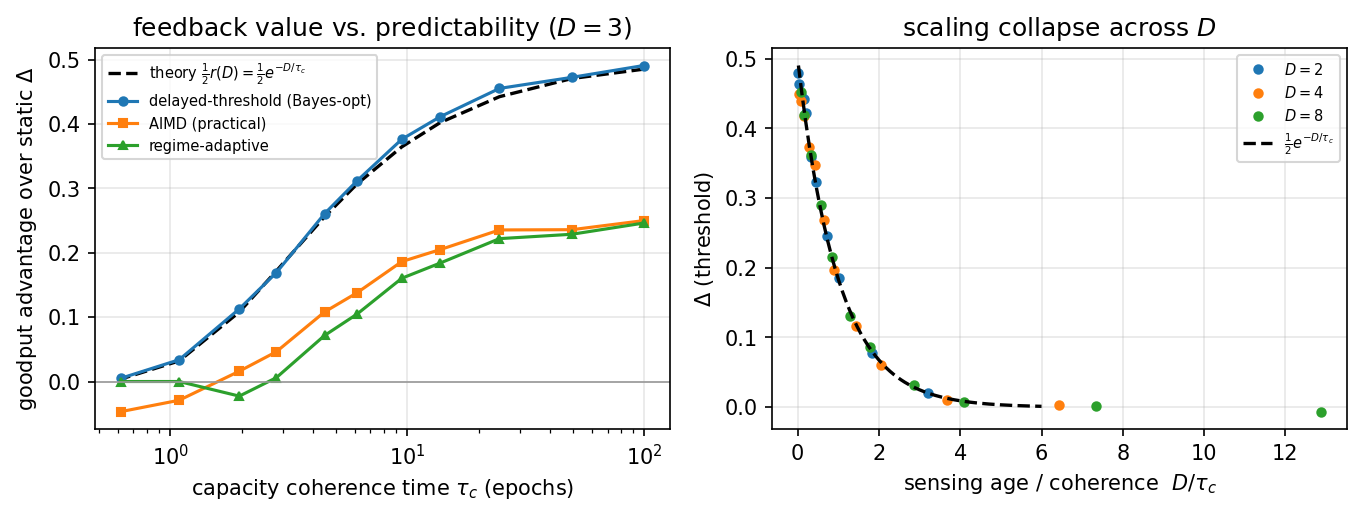
\includegraphics[width=\columnwidth]{figures/tau_sweep.png}
\caption{Controller-level validation. \emph{Left.} Goodput advantage over a fixed
budget against capacity coherence time $\tau_c$ at $D{=}3$. The threshold policy
lies on the predicted $\tfrac12 r(D)$, dashed, to within $0.013$, and the
DeepRM-style policy-gradient agent, diamonds, converges onto it without passing
it. Fixed AIMD falls below a fixed budget once $\tau_c\lesssim D$, and
Algorithm~\ref{alg:adaptive} tracks the envelope. \emph{Right.} Sweeping $D$
collapses the advantage onto $\tfrac12 e^{-D/\tau_c}$ against $D/\tau_c$.}
\label{fig:tausweep}
\end{figure}

\noindent\textbf{Live confirmation on GPU hardware.}
We ran Algorithm~\ref{alg:adaptive} on the same two-GPU node across the Markov
$\tau_c$ sweep, with $p$ from $0.01$ to $0.4$, $D{=}3$ and two seeds, estimating
$r(D)$ online. Two claims transfer from the model. The online estimate lands on
the predicted curve, with $\hat r=(1-2\hat p)^D$ tracking $(1-2p)^D$ to within
$0.07$ (Fig.~\ref{fig:e9adapt}, left). And the switch modulates as predicted, its
closed-loop fraction falling from $0.98$ to $0.48$ as $r(D)$ drops past $\theta$.
Hardware differs from simulation in one instructive way. Raw goodput rewards
over-admission, so live AIMD out-performs a fixed budget everywhere, and at high
flip rate it buys that goodput with impoliteness at $\rho=0.44$ against $0.04$
rather than by tracking. The predicted crossover therefore does not appear in raw
goodput. It appears on the goodput and politeness frontier
(Fig.~\ref{fig:e9adapt}, right) as the over-admission the switch sheds against
always running AIMD, which grows from $+0.01$ to $+0.22$ as $p$ rises from $0.08$
to $0.4$. Algorithm~\ref{alg:adaptive} matches AIMD where the neighbour is
trackable and recovers a fixed budget's politeness where it is not.

\begin{figure}[t]
\centering
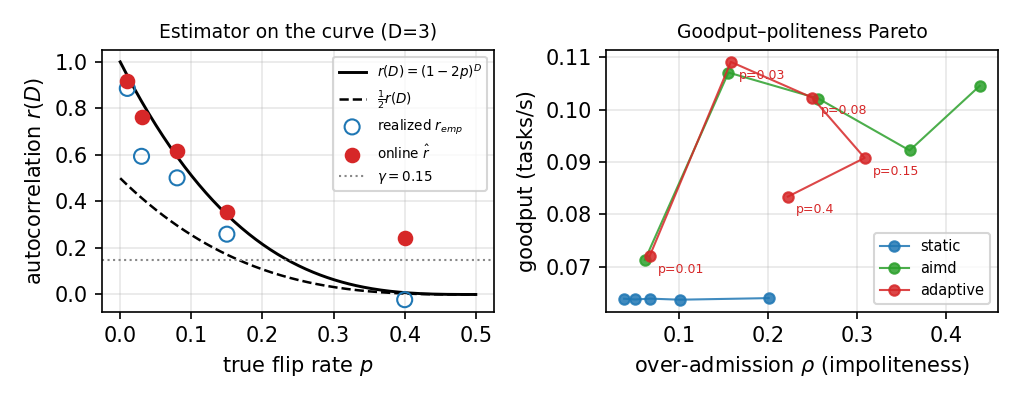
\includegraphics[width=\columnwidth]{figures/e9_adaptive_curve.png}
\caption{Algorithm~\ref{alg:adaptive} live on two GV100 GPUs, Markov $\tau_c$
sweep, $D{=}3$, two seeds. \emph{Left.} The online estimate $\hat r$ and the
realized availability autocorrelation land on $(1-2p)^D$, and the switch fires as
$r(D)$ crosses $\theta$. \emph{Right.} The goodput and over-admission frontier,
where the adaptive controller tracks AIMD when feedback is useful and moves toward
a fixed budget's politeness as $p$ grows.}
\label{fig:e9adapt}
\end{figure}

\subsection{Summary and threats to validity}
\label{sec:eval-threats}
The evaluation establishes four things. The sensing age is a measured first-order
term at about $2.5$\,s, dominated by CUDA start-up. Under a self-imposed budget
Algorithm~\ref{alg:adaptive} delivers $1.7$ to $3.2$ times a fixed rate's goodput
at $\rho=0$. Under structured contention it is the polite and efficient knee and
spares the neighbour, while under memoryless contention feedback breaks even, a
pre-registered null we report rather than suppress. And the value
$\tfrac12 r(D)$ holds at the controller level, with the threshold policy on it to
within $0.013$, a learned policy-gradient agent capped by it, and
Algorithm~\ref{alg:adaptive} never below a fixed budget, which unifies the two
live contention cases as endpoints of one curve.

Three threats remain. Contention is manufactured on a two-GPU node at $C{=}2$ with
synthetic profiles rather than drawn from a production multi-tenant trace. The
clean tracing of the advantage in Q4 is controller-level, because live static is a
fixed trickle with no tunable frontier to measure an advantage against. And the
live adaptive sweep uses two seeds per point, so it is a confirmatory anchor
rather than primary evidence. The full system path is nonetheless verified
end-to-end in \S\ref{sec:impl}, and naive's impoliteness, at $\rho\ge0.64$ with at
least $38\%$ neighbour harm, is robust across every case.
